\documentclass{beamer}

\usefonttheme{professionalfonts} % using non standard fonts for beamer
\usefonttheme{serif} % default family is serif

\usepackage{hyperref}

%\usepackage{minted}

\usepackage{animate}

\usepackage{graphicx}

\def\Put(#1,#2)#3{\leavevmode\makebox(0,0){\put(#1,#2){#3}}}

\usepackage{color}

\usepackage{tikz}

\usepackage{amssymb}

\usepackage{enumerate}


\newcommand\blfootnote[1]{%

  \begingroup

  \renewcommand\thefootnote{}\footnote{#1}%

  \addtocounter{footnote}{-1}%

  \endgroup

}

\makeatletter

%%%%%%%%%%%%%%%%%%%%%%%%%%%%%% Textclass specific LaTeX commands.

 % this default might be overridden by plain title style

 \newcommand\makebeamertitle{\frame{\maketitle}}%

 % (ERT) argument for the TOC

 \AtBeginDocument{%

   \let\origtableofcontents=\tableofcontents

   \def\tableofcontents{\@ifnextchar[{\origtableofcontents}{\gobbletableofcontents}}

   \def\gobbletableofcontents#1{\origtableofcontents}

 }

%%%%%%%%%%%%%%%%%%%%%%%%%%%%%% User specified LaTeX commands.

\usetheme{Malmoe}

% or ...

\useoutertheme{infolines}

\addtobeamertemplate{headline}{}{\vskip2pt}



\setbeamercovered{transparent}

% or whatever (possibly just delete it)

\makeatother

\begin{document}
\title[DCEL report]{Parallel DCEL Construction Report}
\author[AC]{Andres Calderon}
\institute[Summer'19]{University of California, Riverside}
\makebeamertitle
\newif\iflattersubsect

\AtBeginSection[] {
    \begin{frame}<beamer>
    \frametitle{Outline} 
    \tableofcontents[currentsection]  
    \end{frame}
    \lattersubsectfalse
}

\AtBeginSubsection[] {
    \begin{frame}<beamer>
    \frametitle{Outline} 
    \tableofcontents[currentsubsection]  
    \end{frame}
}

\begin{frame}{Parallel DCEL construction}
    \centering 
    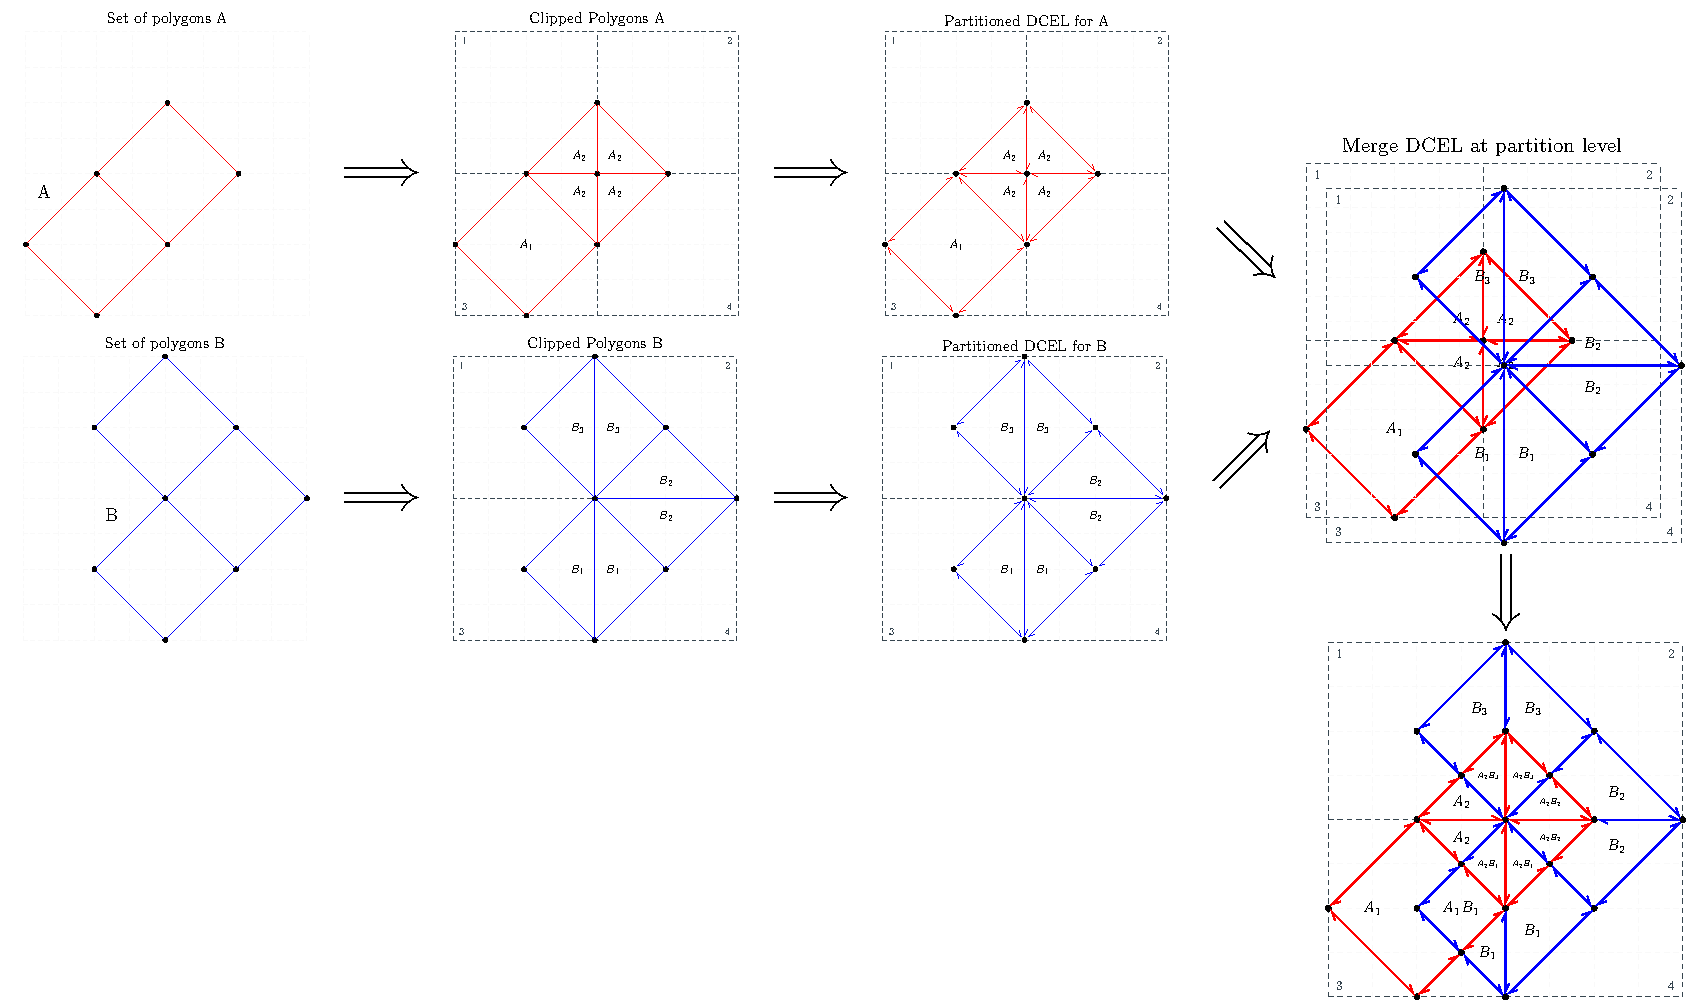
\includegraphics[width=\linewidth]{figures/OverlayParted1} 
\end{frame}

\begin{frame}{Parallel DCEL operations}
    \centering 
    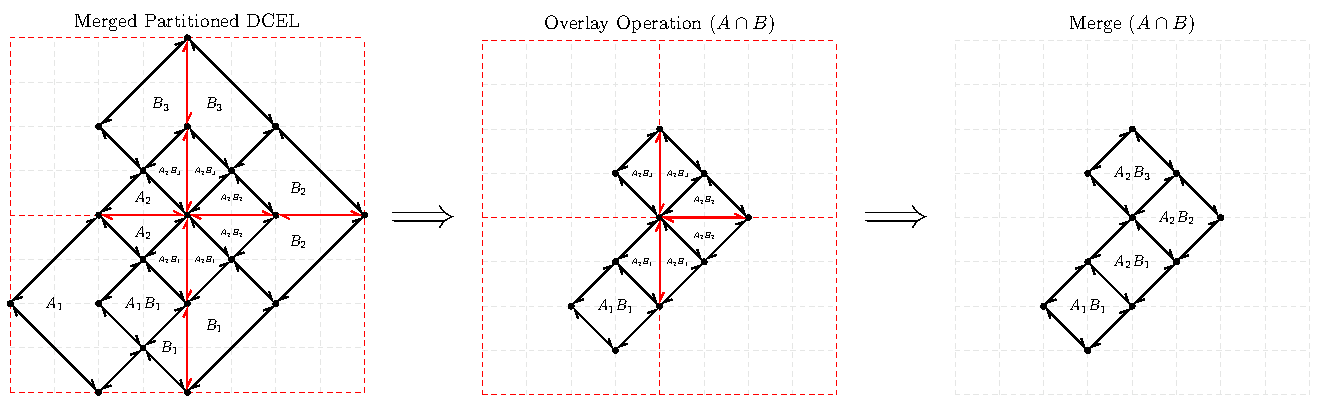
\includegraphics[width=\linewidth]{figures/OverlayParted2} 
\end{frame}

\begin{frame}{Phili test [2000]}
    \centering 
    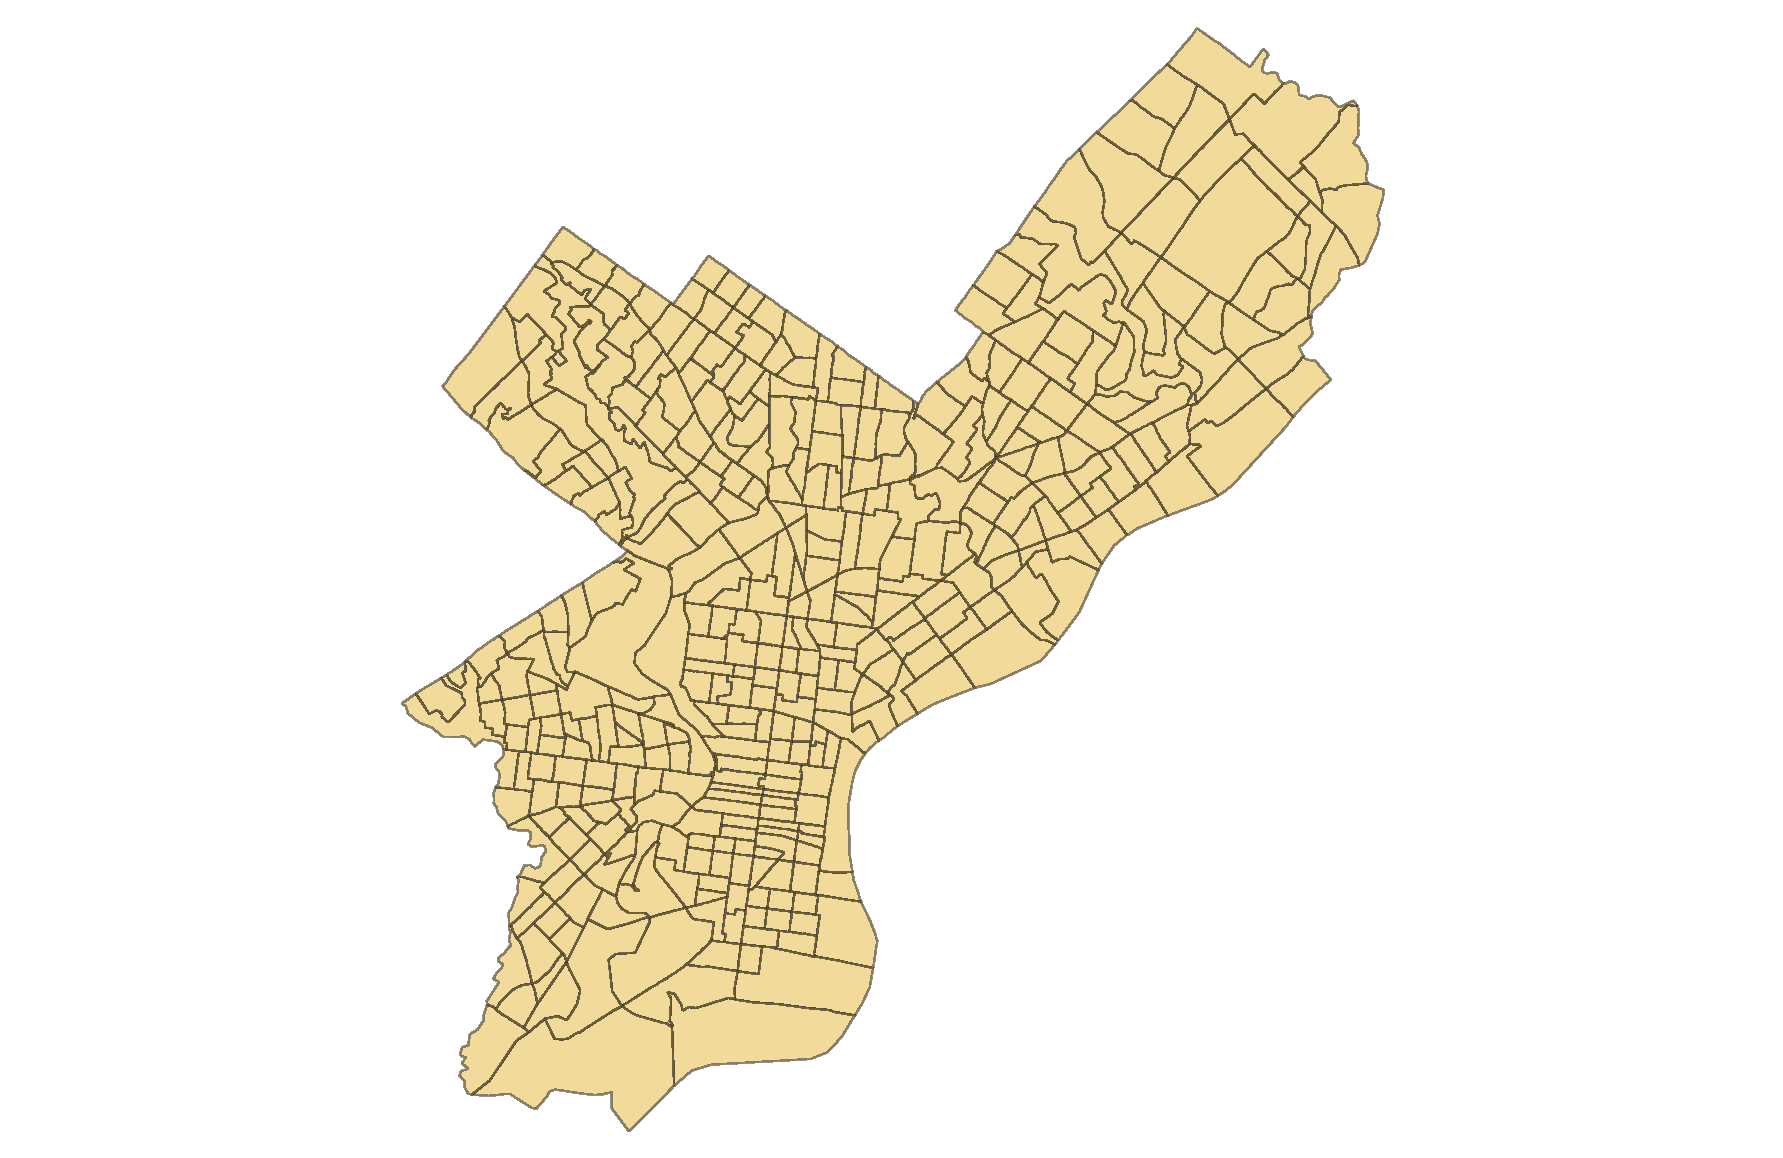
\includegraphics[trim=6cm 0cm 6cm 0cm, clip, width=0.6\linewidth]{figures/phili2000} 
\end{frame}

\begin{frame}{Phili test [2010]}
    \centering 
    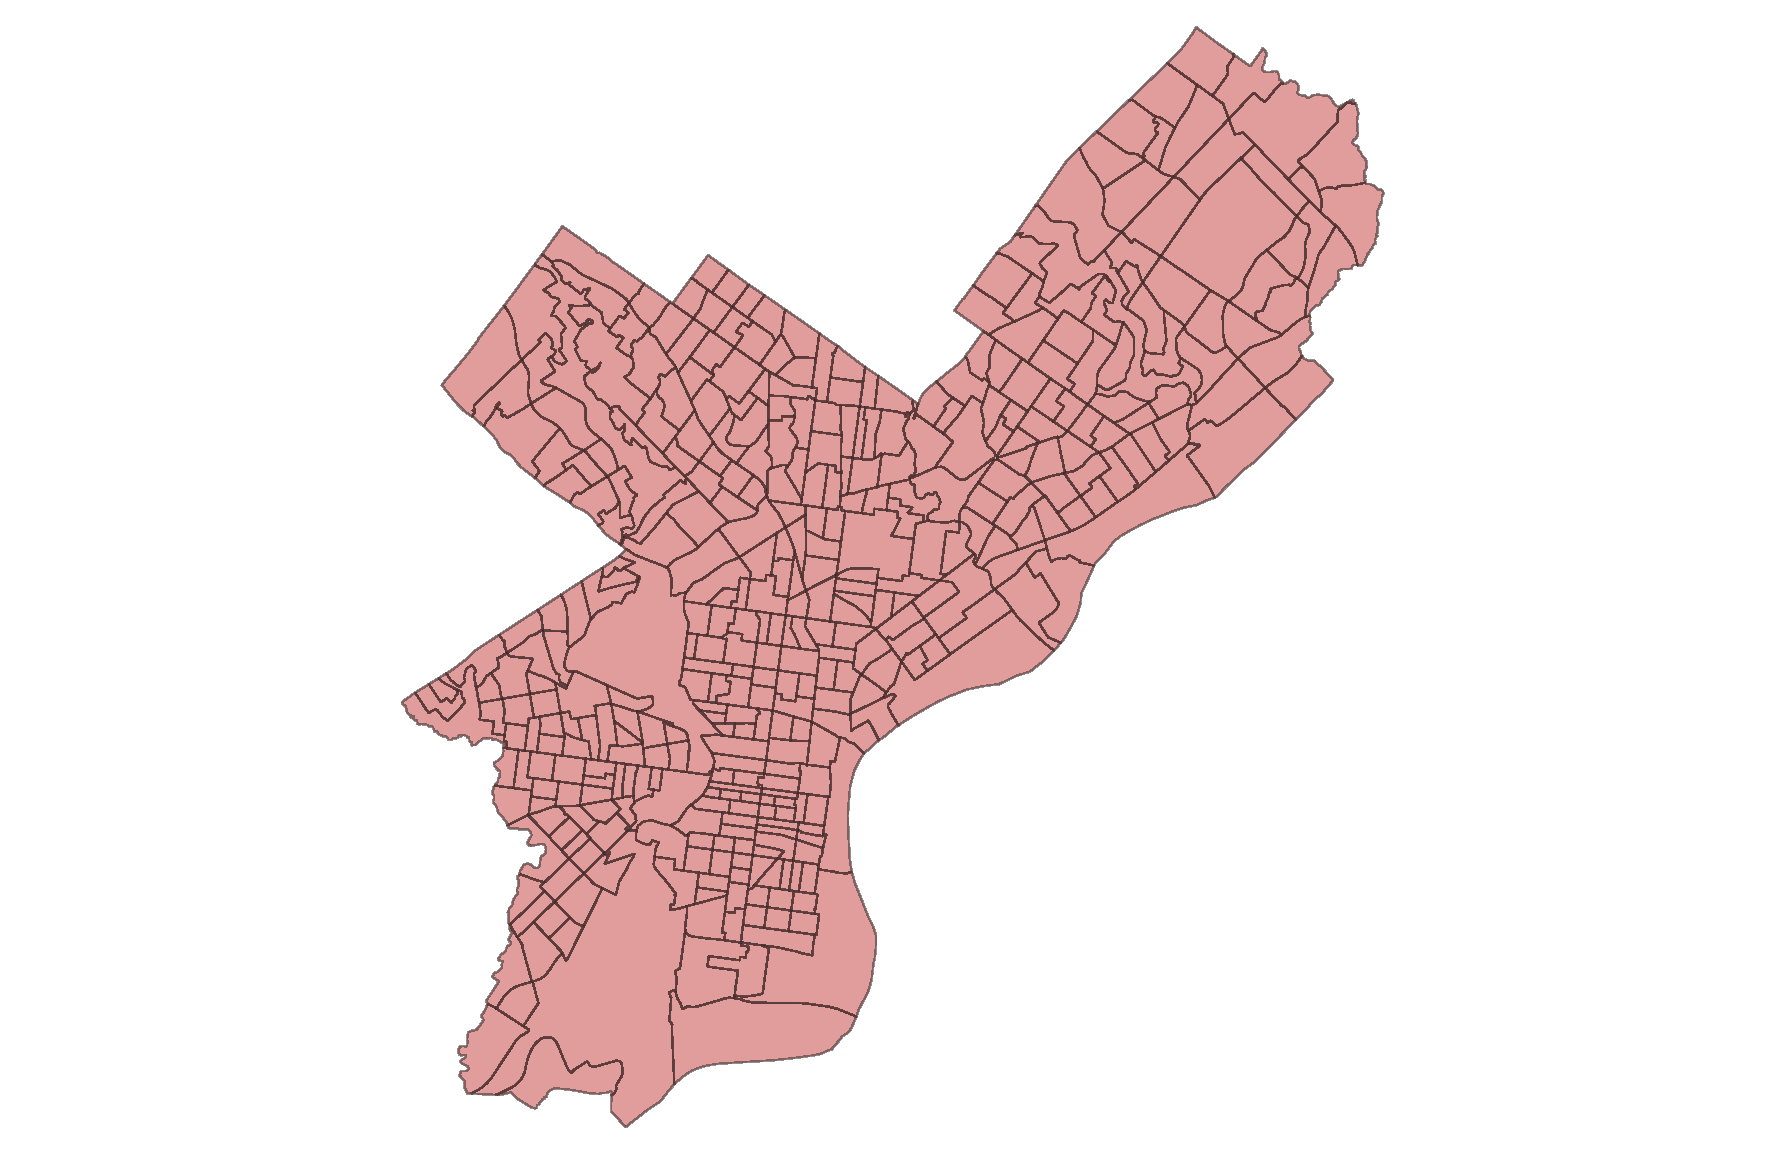
\includegraphics[trim=6cm 0cm 6cm 0cm, clip, width=0.6\linewidth]{figures/phili2010} 
\end{frame}

\begin{frame}{Phili test [Merged DCEL]}
    \centering 
    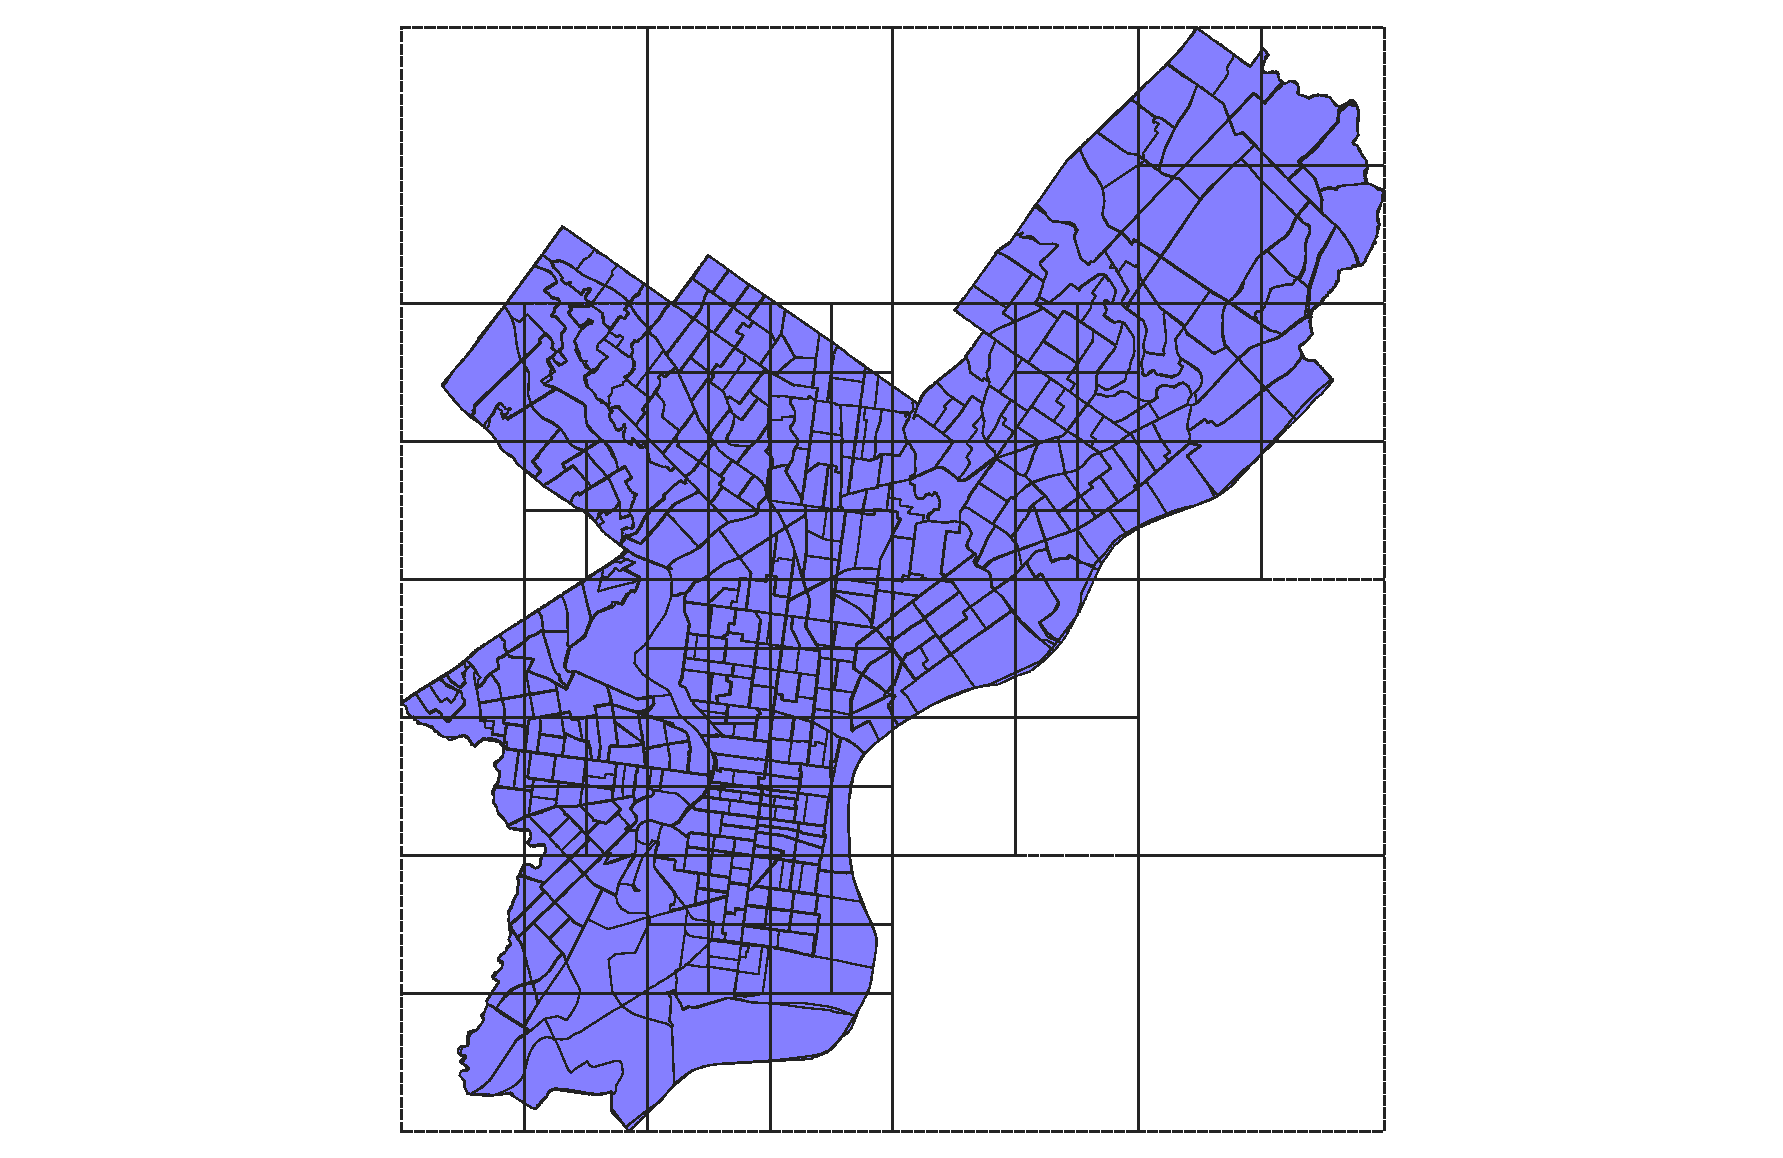
\includegraphics[trim=6cm 0cm 6cm 0cm, clip, width=0.6\linewidth]{figures/faces} 
\end{frame}

\begin{frame}{Phili test [Union]}
    \centering 
    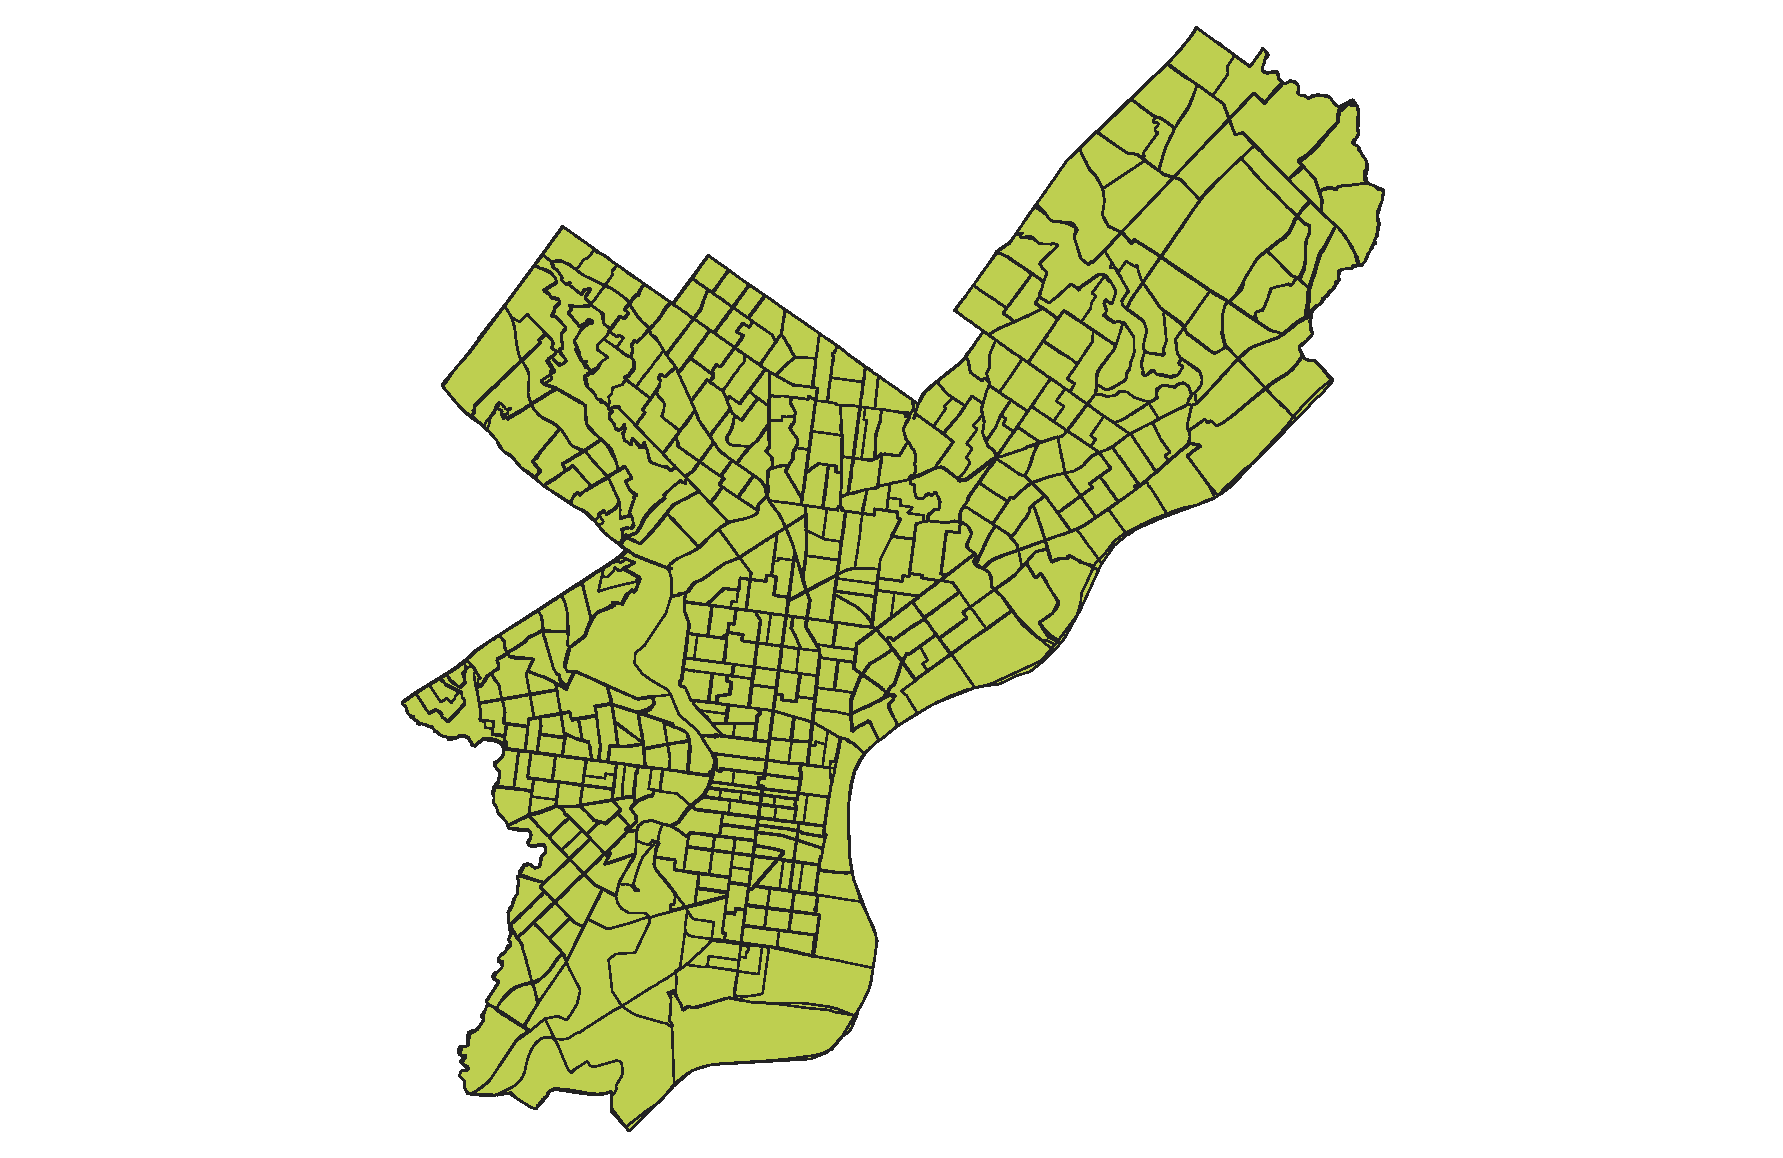
\includegraphics[trim=6cm 0cm 6cm 0cm, clip, width=0.6\linewidth]{figures/union} 
\end{frame}
\begin{frame}{Phili test [Intersection]}
    \centering 
    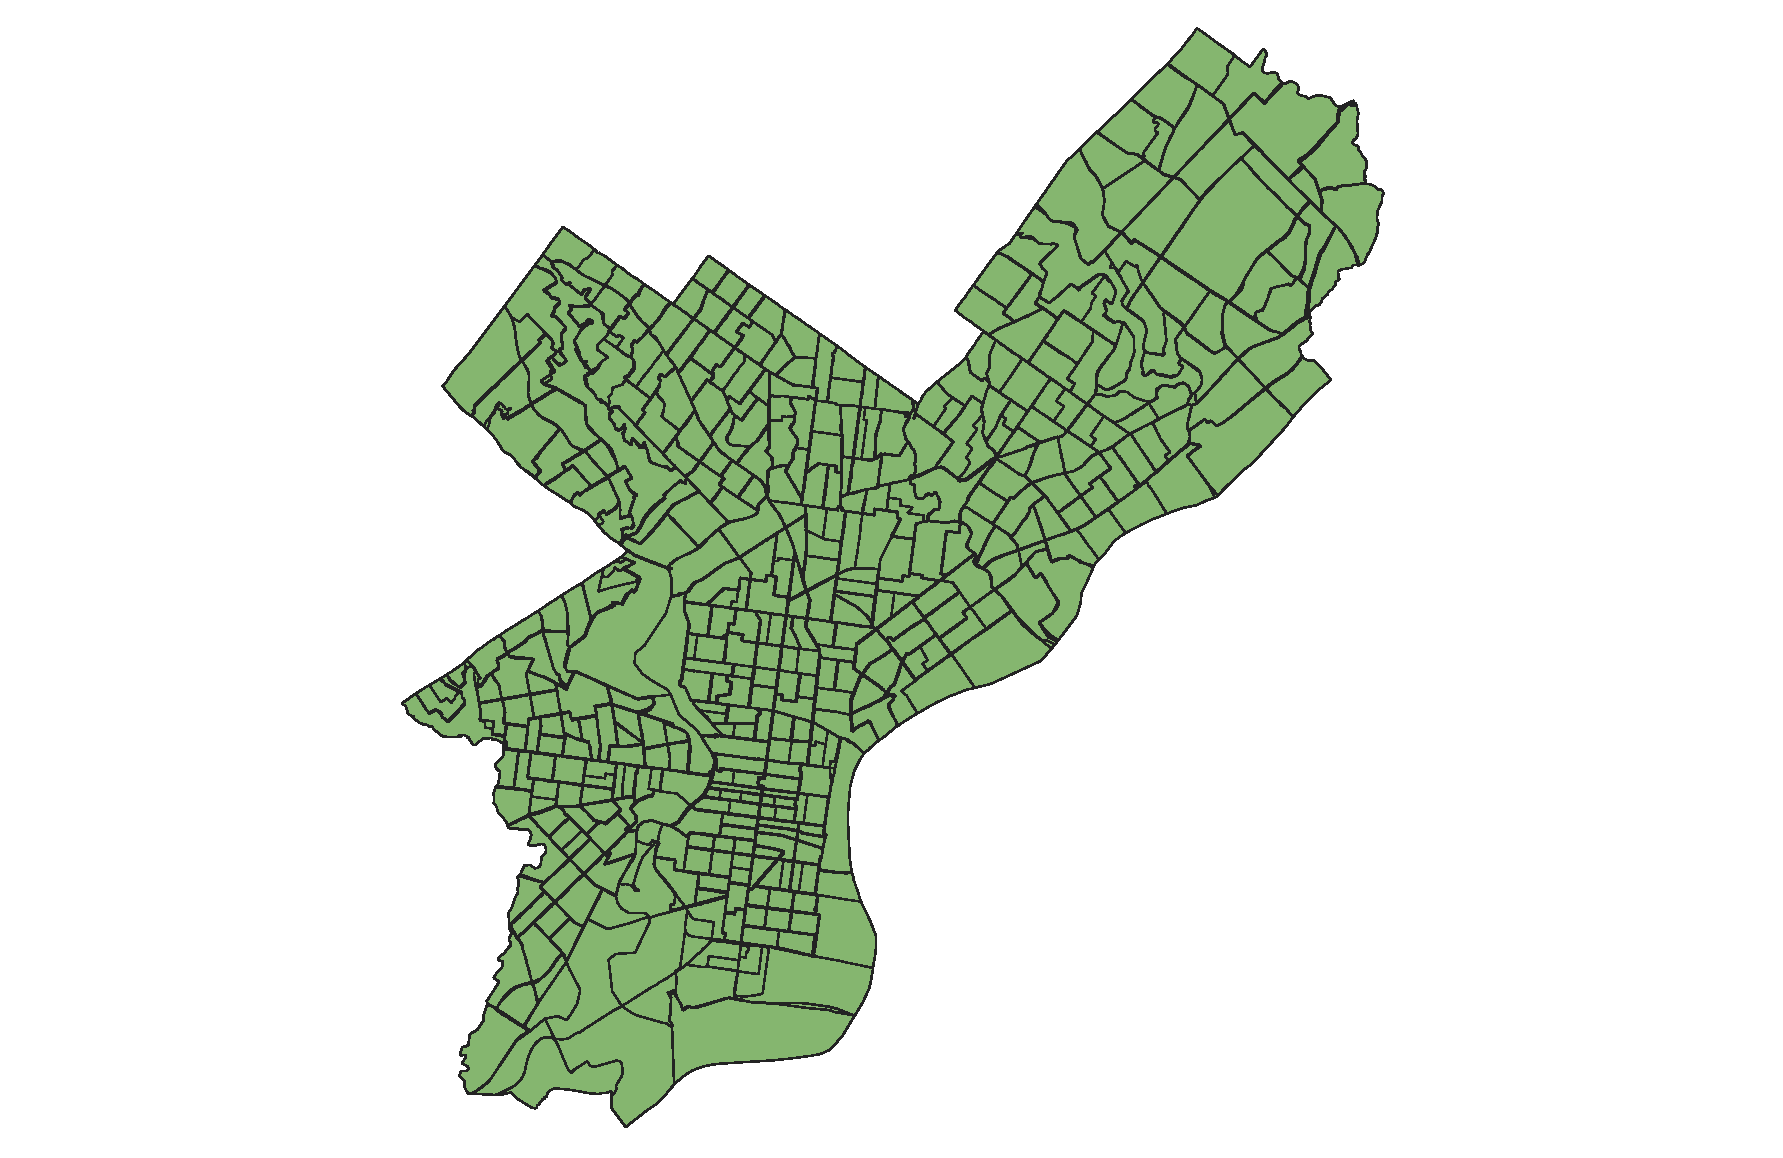
\includegraphics[trim=6cm 0cm 6cm 0cm, clip, width=0.6\linewidth]{figures/intersection} 
\end{frame}
\begin{frame}{Phili test [Symmetric difference]}
    \centering 
    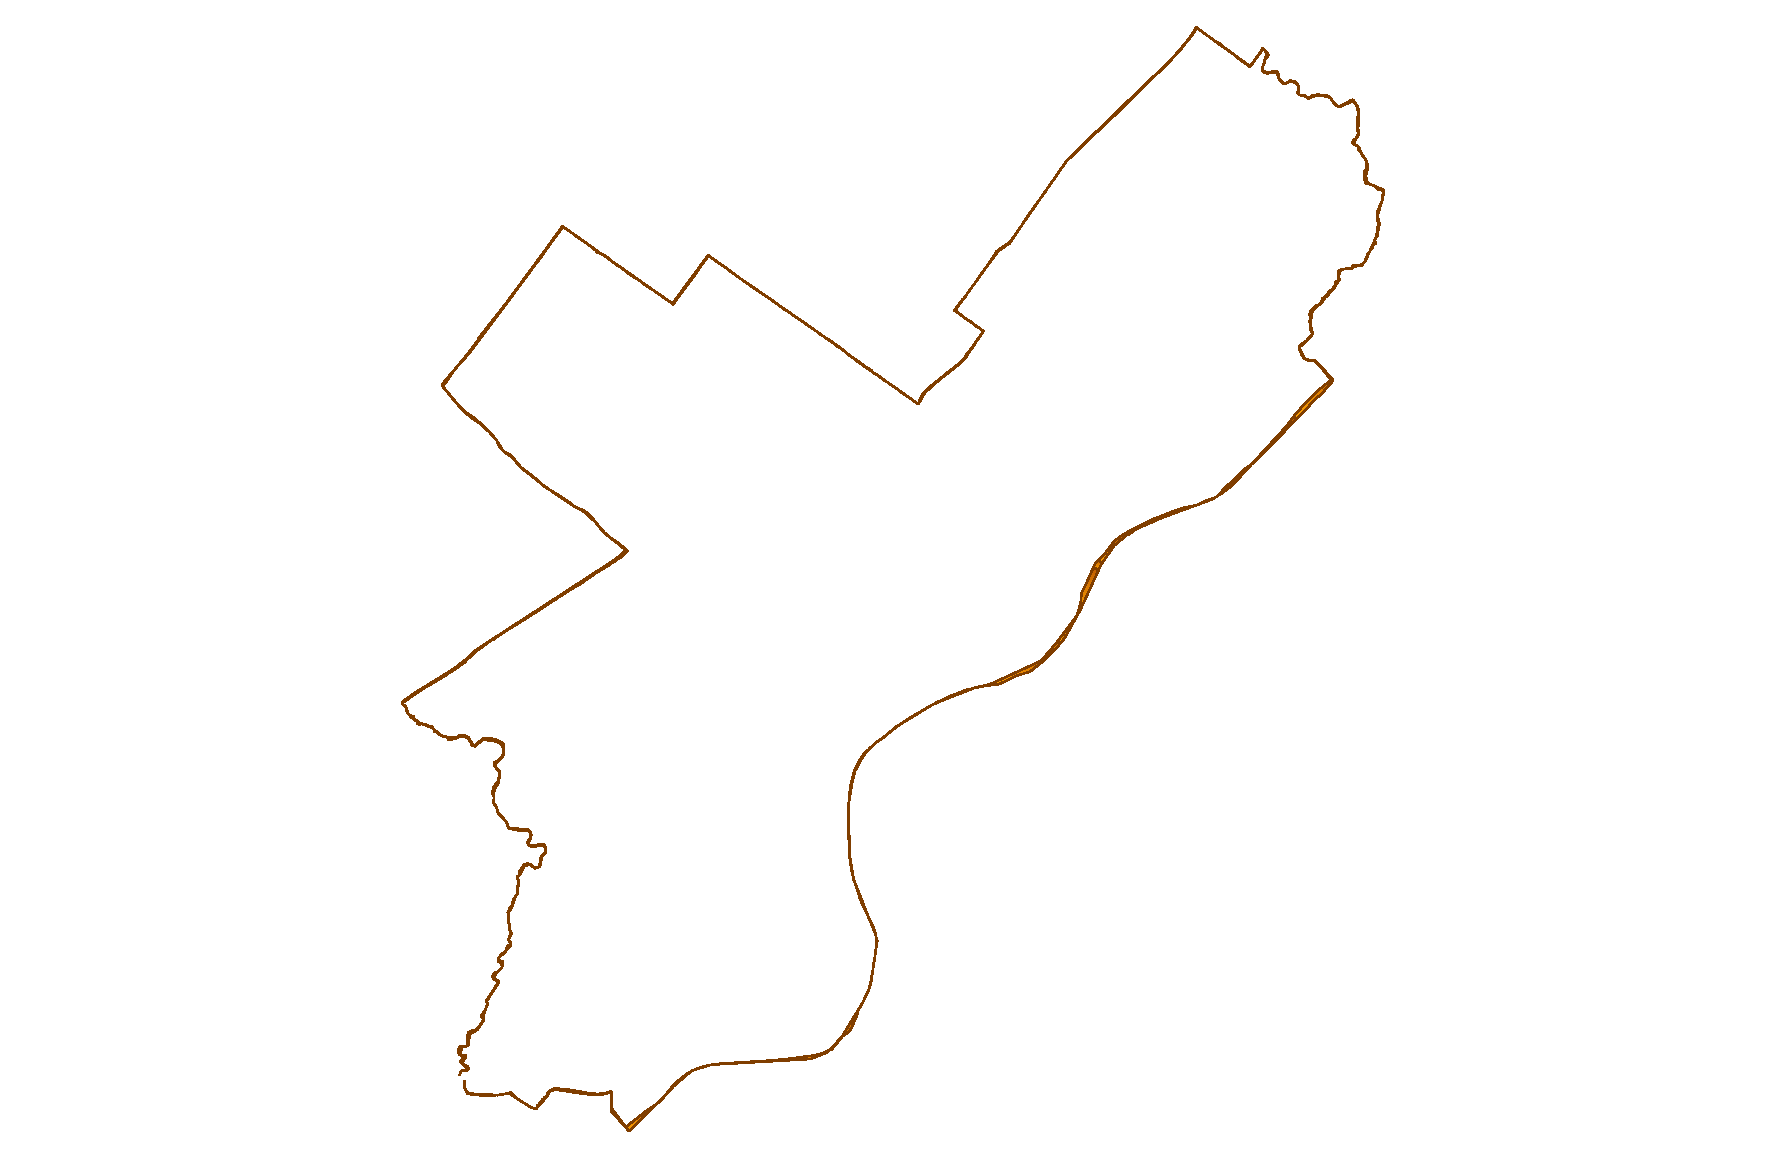
\includegraphics[trim=6cm 0cm 6cm 0cm, clip, width=0.6\linewidth]{figures/symmetric} 
\end{frame}
\begin{frame}{Phili test [Difference ($A \setminus B$)]}
    \centering 
    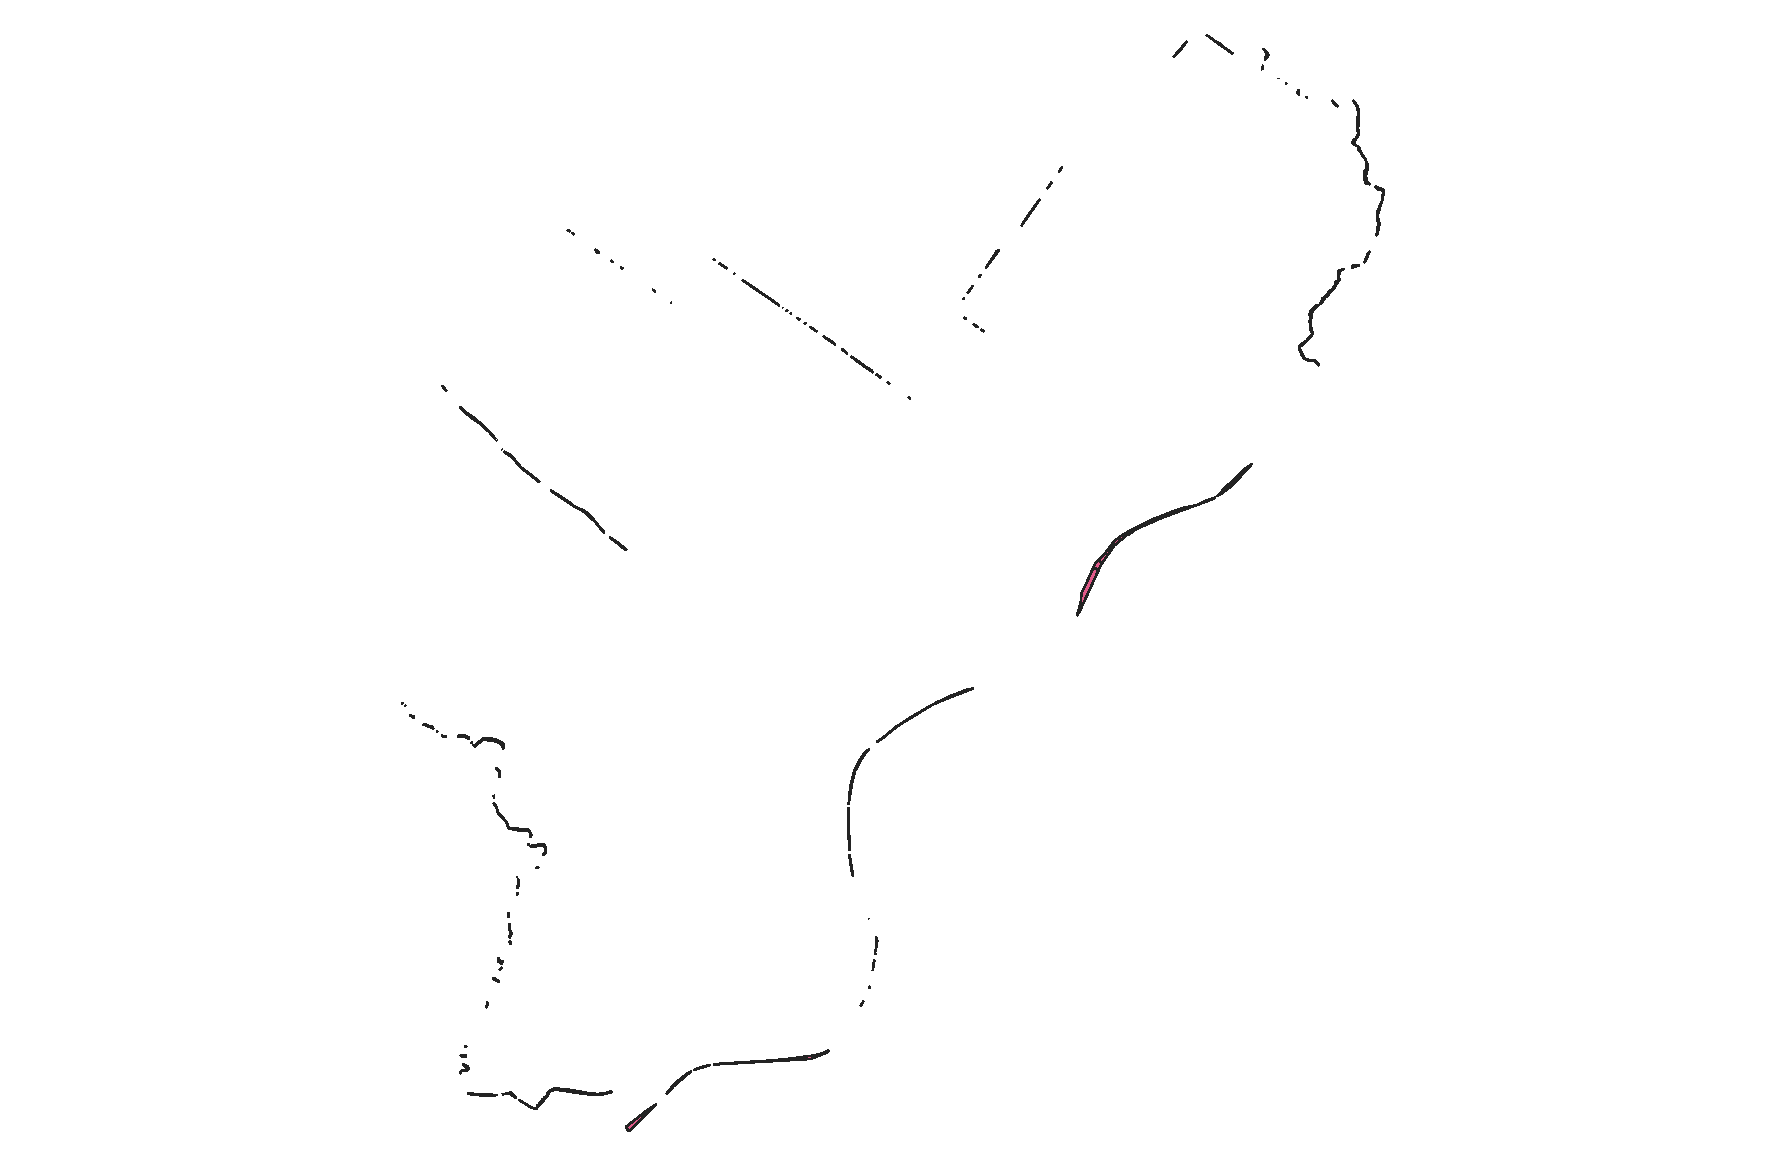
\includegraphics[trim=6cm 0cm 6cm 0cm, clip, width=0.6\linewidth]{figures/differenceA} 
\end{frame}
\begin{frame}{Phili test [Difference ($B \setminus A$)]}
    \centering 
    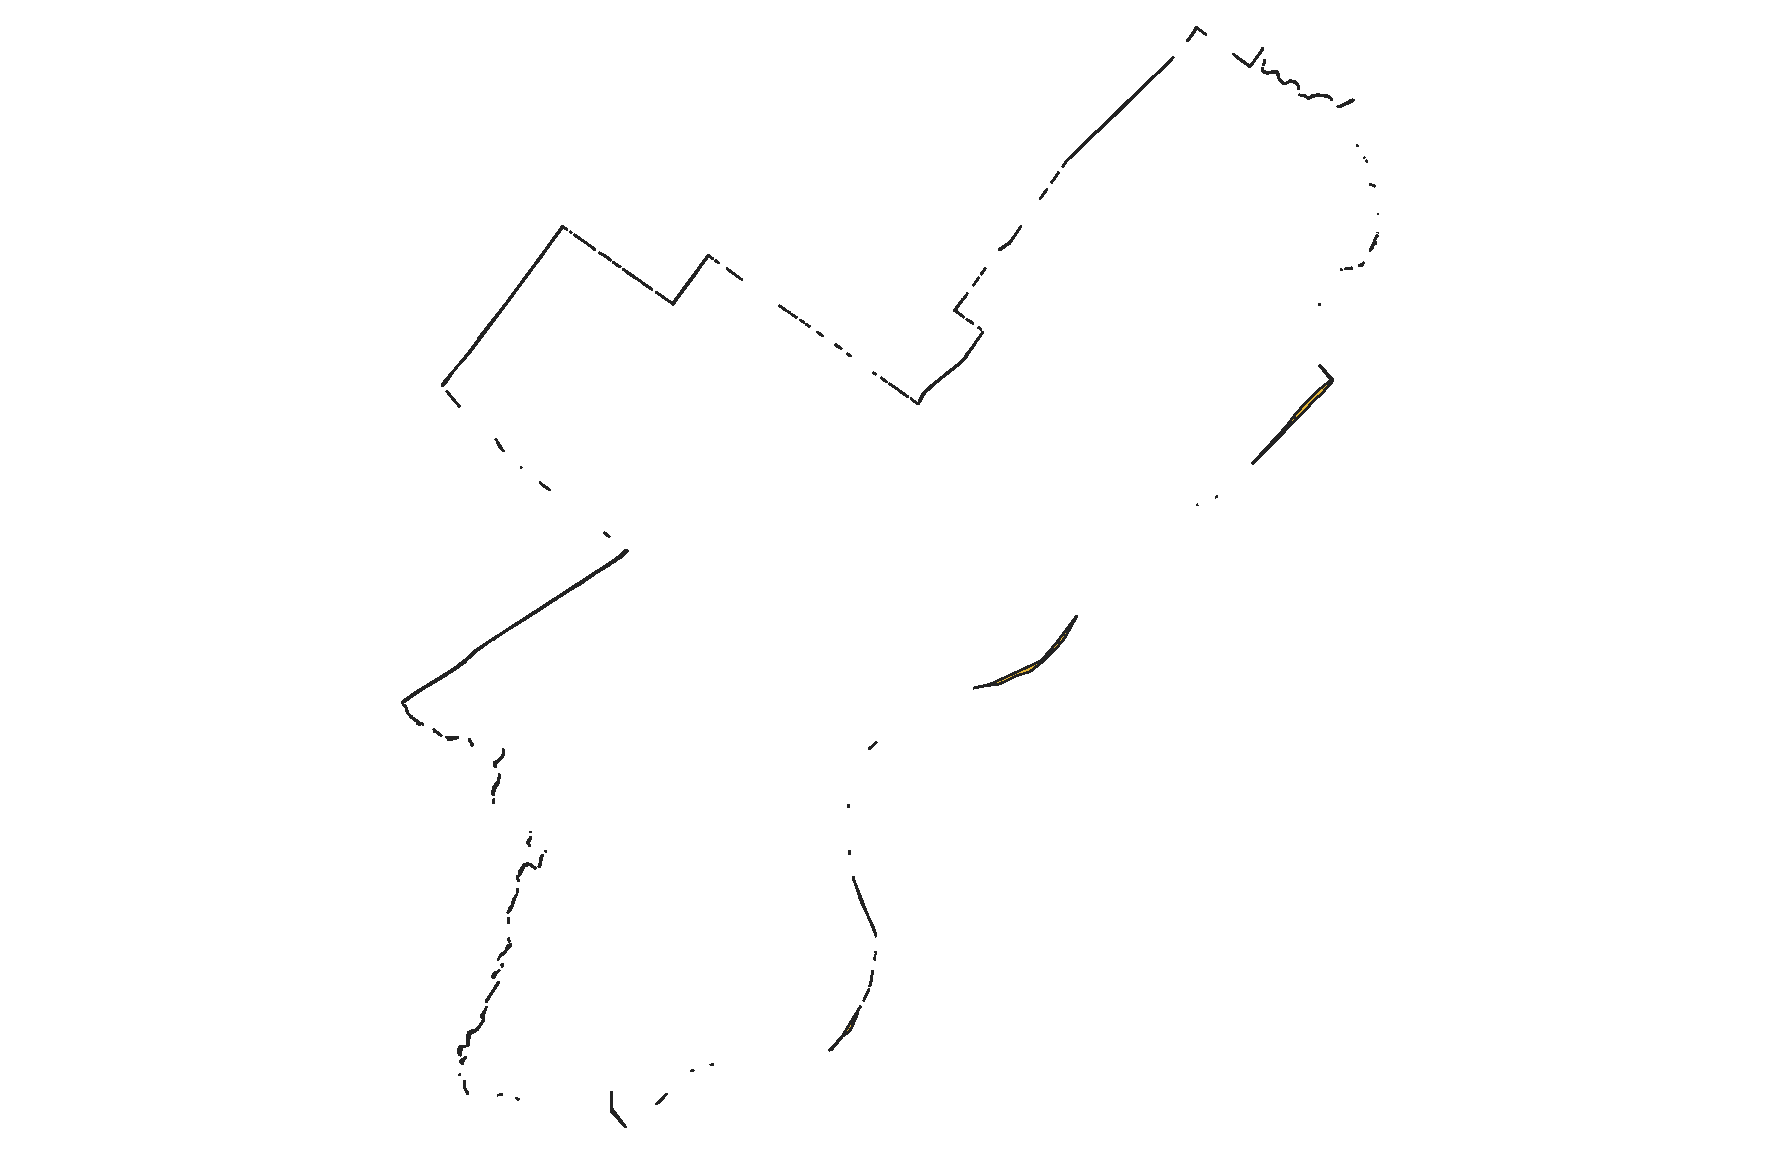
\includegraphics[trim=6cm 0cm 6cm 0cm, clip, width=0.6\linewidth]{figures/differenceB} 
\end{frame}

\begin{frame}{Phili test [Performance]}
    \centering 
    \begin{tabular}{|c|c|c|}
        \hline
                        & Parallel DCEL & QGIS \\ \hline
        Partitioning    & 0.55  & - \\
        Clipping        & 1.96  & - \\
        Local DCEL      & 2.68  & - \\
        Merged DCEL     & 1.62  & - \\ \hline
        Union           & 0.89  & 7.41 \\
        Intersection    & 0.60  & 4.56 \\
        Symmetric       & 0.43  & 3.84 \\
        Difference A    & 0.34  & 1.68 \\
        Difference B    & 0.39  & 2.19 \\ \hline
        Total           & 9.46  & 19.68 \\ \hline
    \end{tabular}    
\end{frame}

\begin{frame}{Working with holes}
    \centering 
    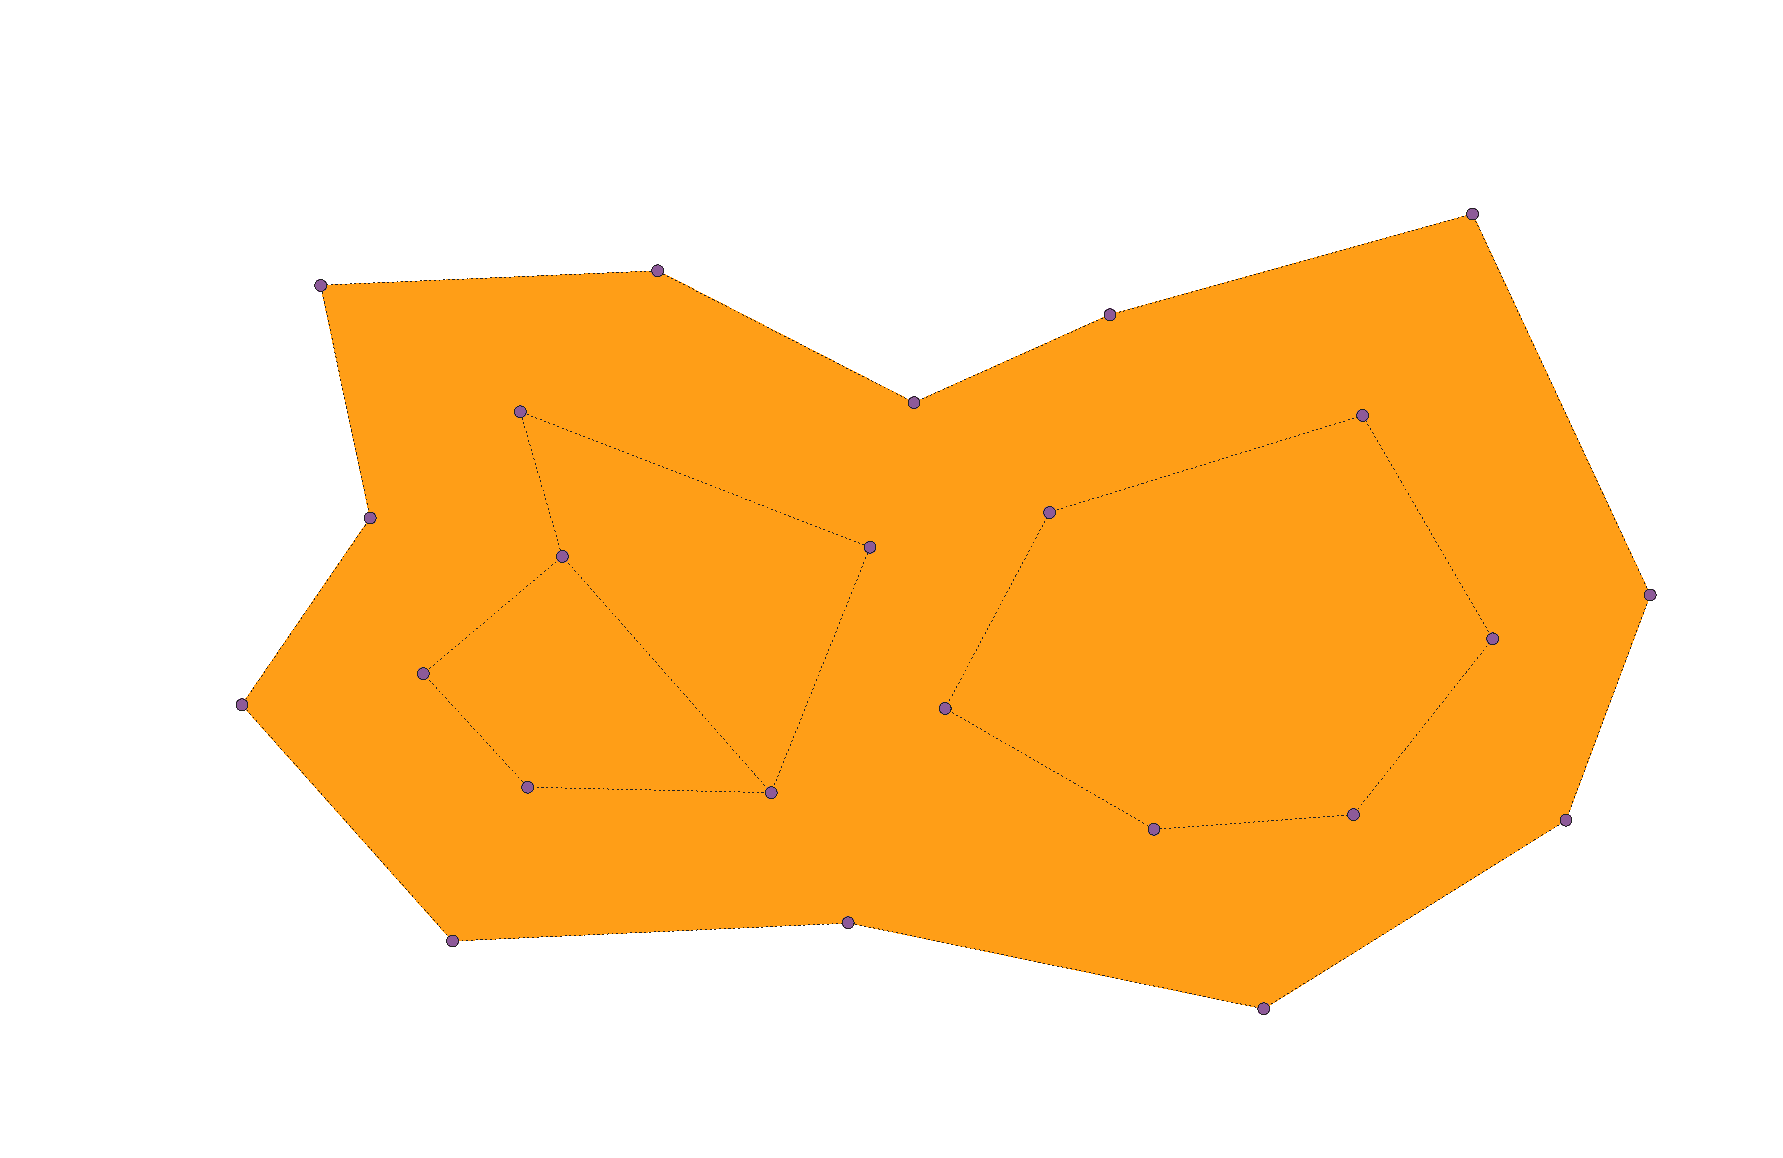
\includegraphics[trim=3cm 0cm 2cm 0cm, clip, width=0.75\linewidth]{figures/Holes01} 
\end{frame}
\begin{frame}{Working with holes}
    \centering 
    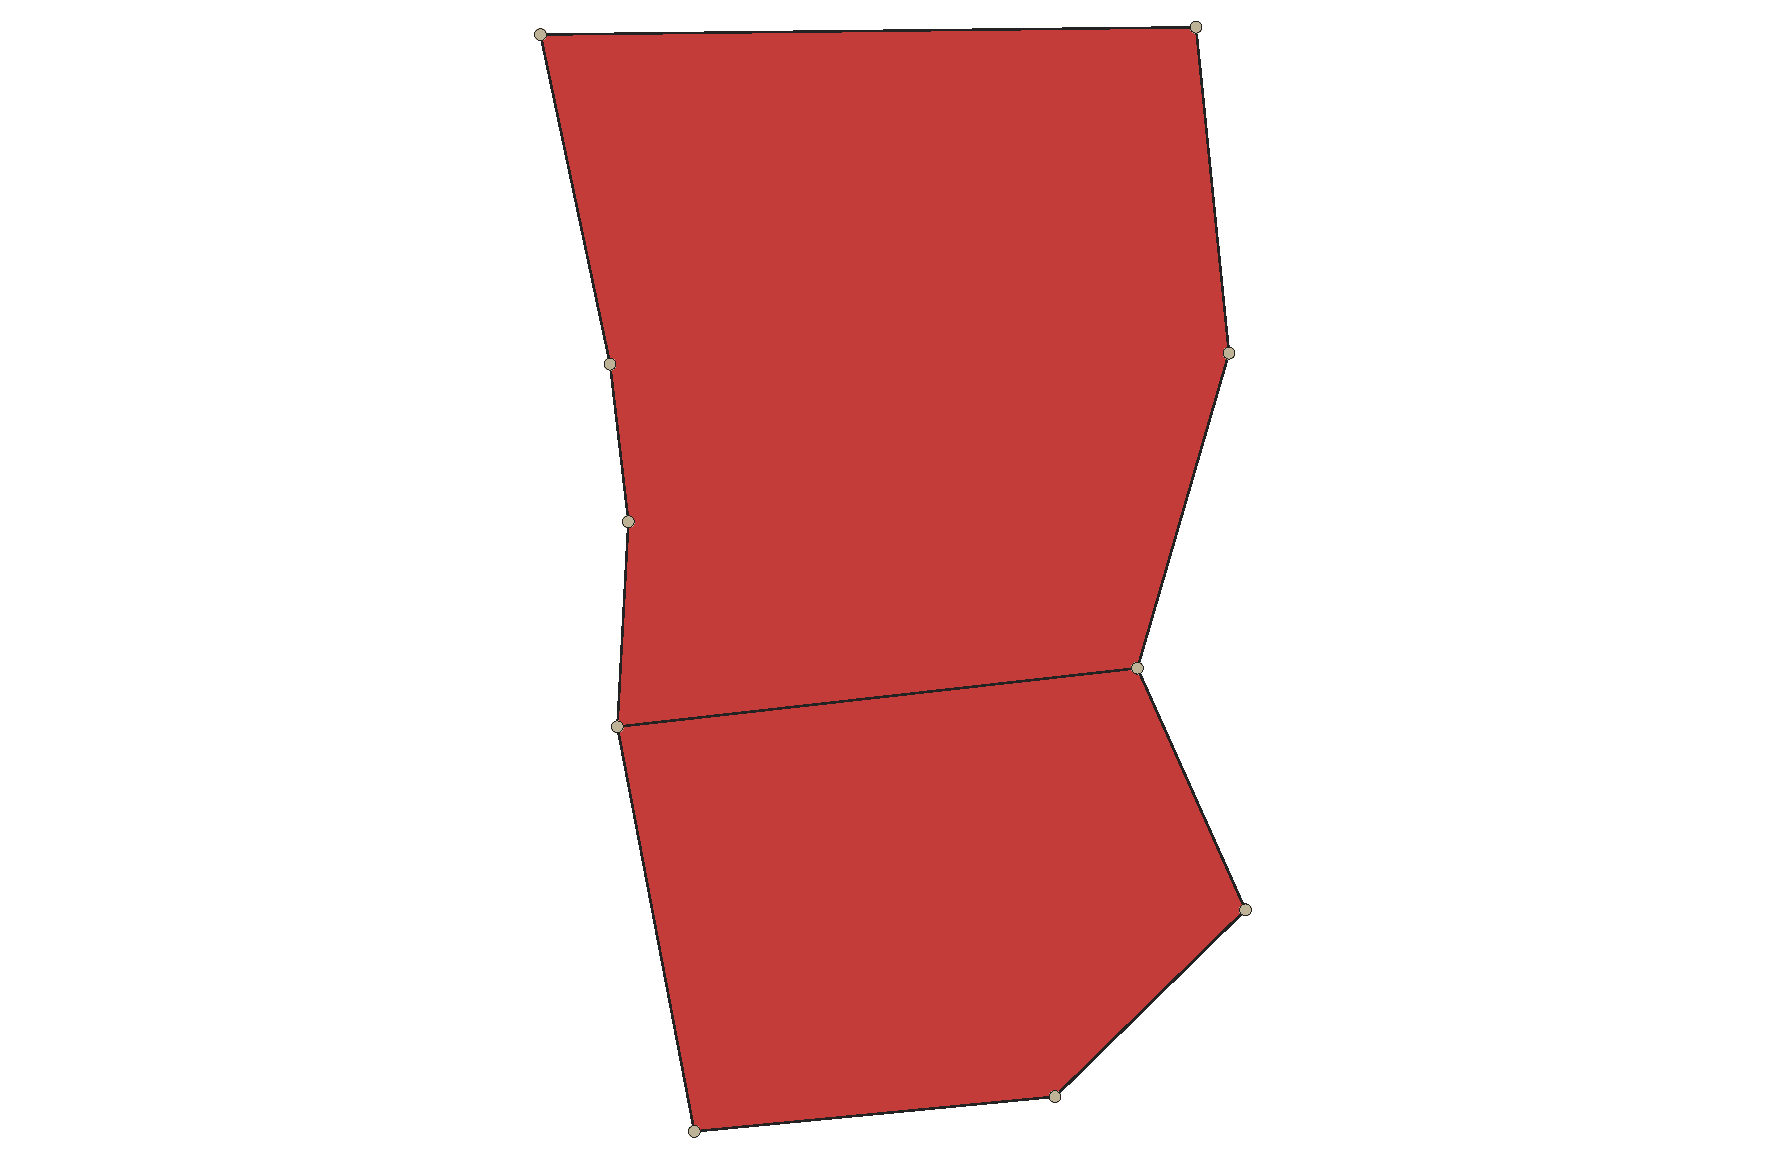
\includegraphics[trim=3cm 0cm 2cm 0cm, clip, width=0.75\linewidth]{figures/Holes02} 
\end{frame}
\begin{frame}{Merged DCEL}
    \centering 
    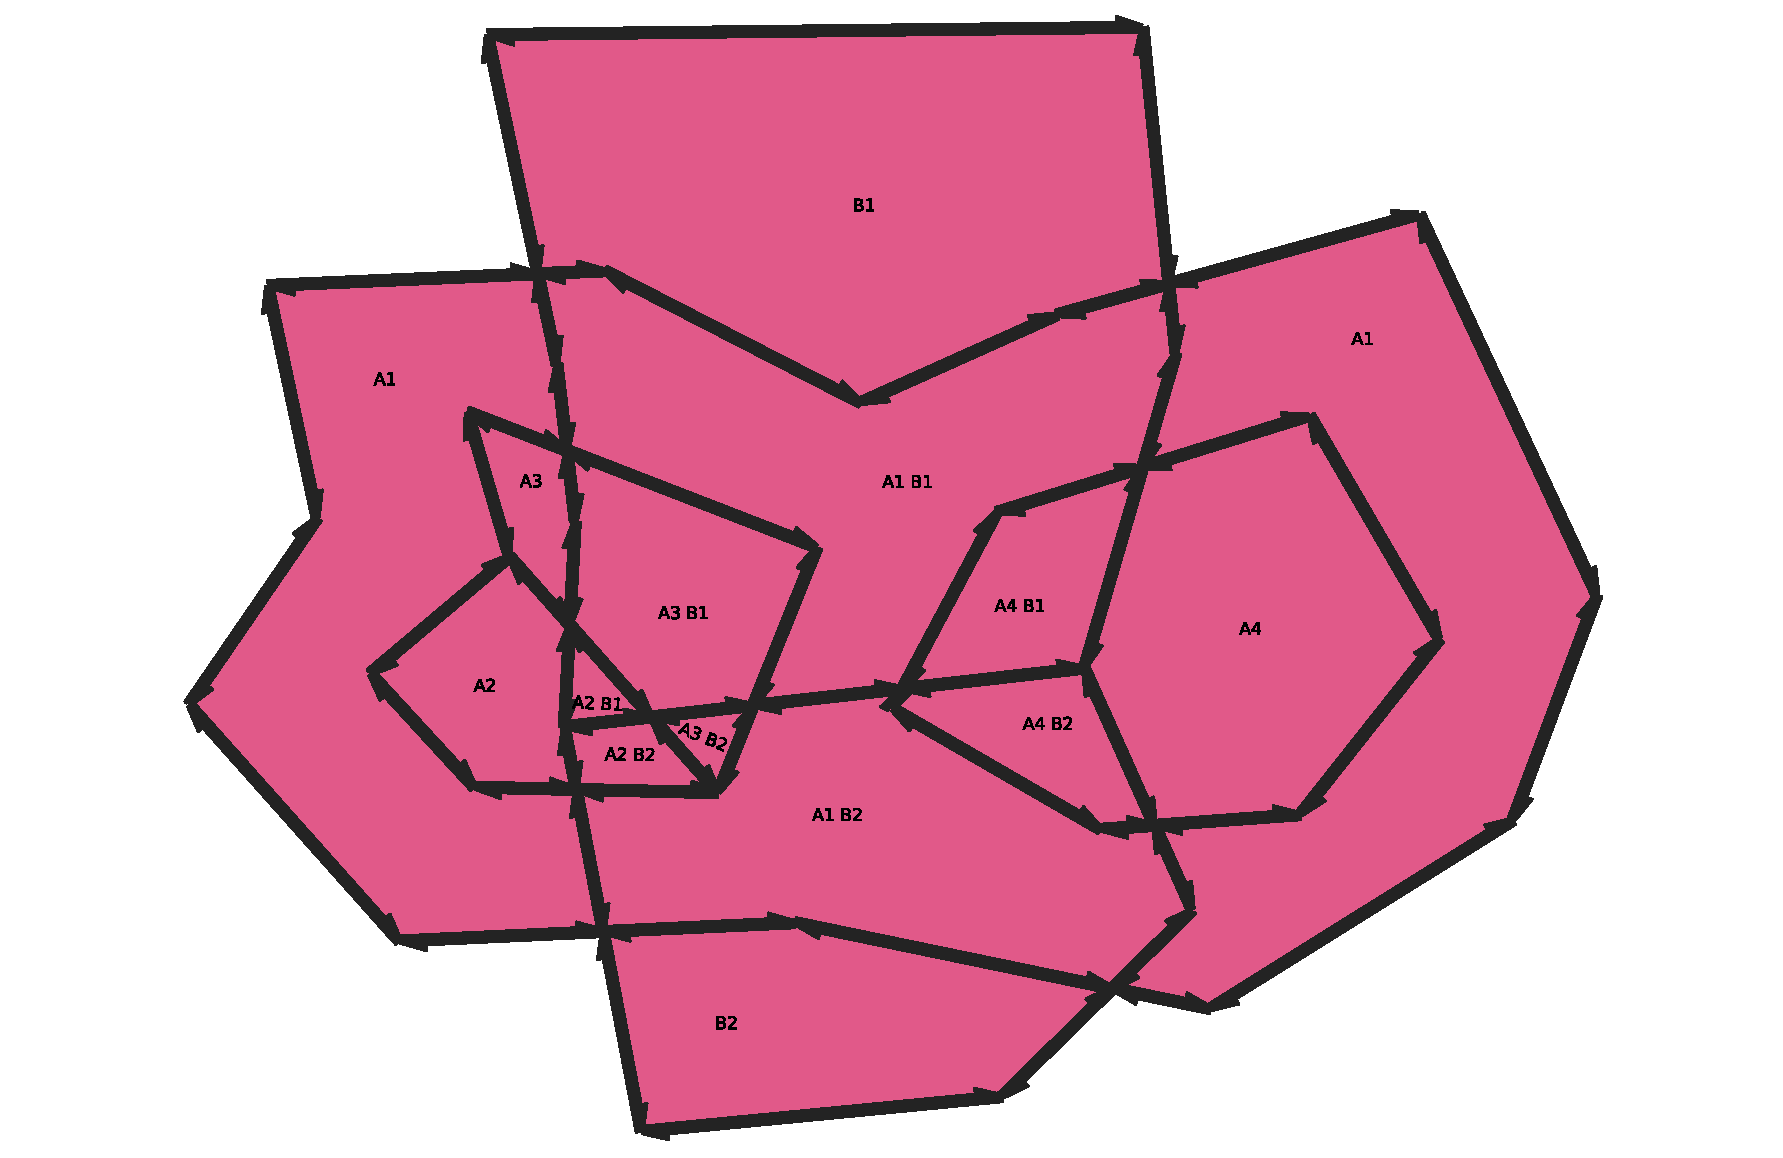
\includegraphics[trim=3cm 0cm 2cm 0cm, clip, width=0.75\linewidth]{figures/Holes03} 
\end{frame}
\begin{frame}{Intersection}
    \centering 
    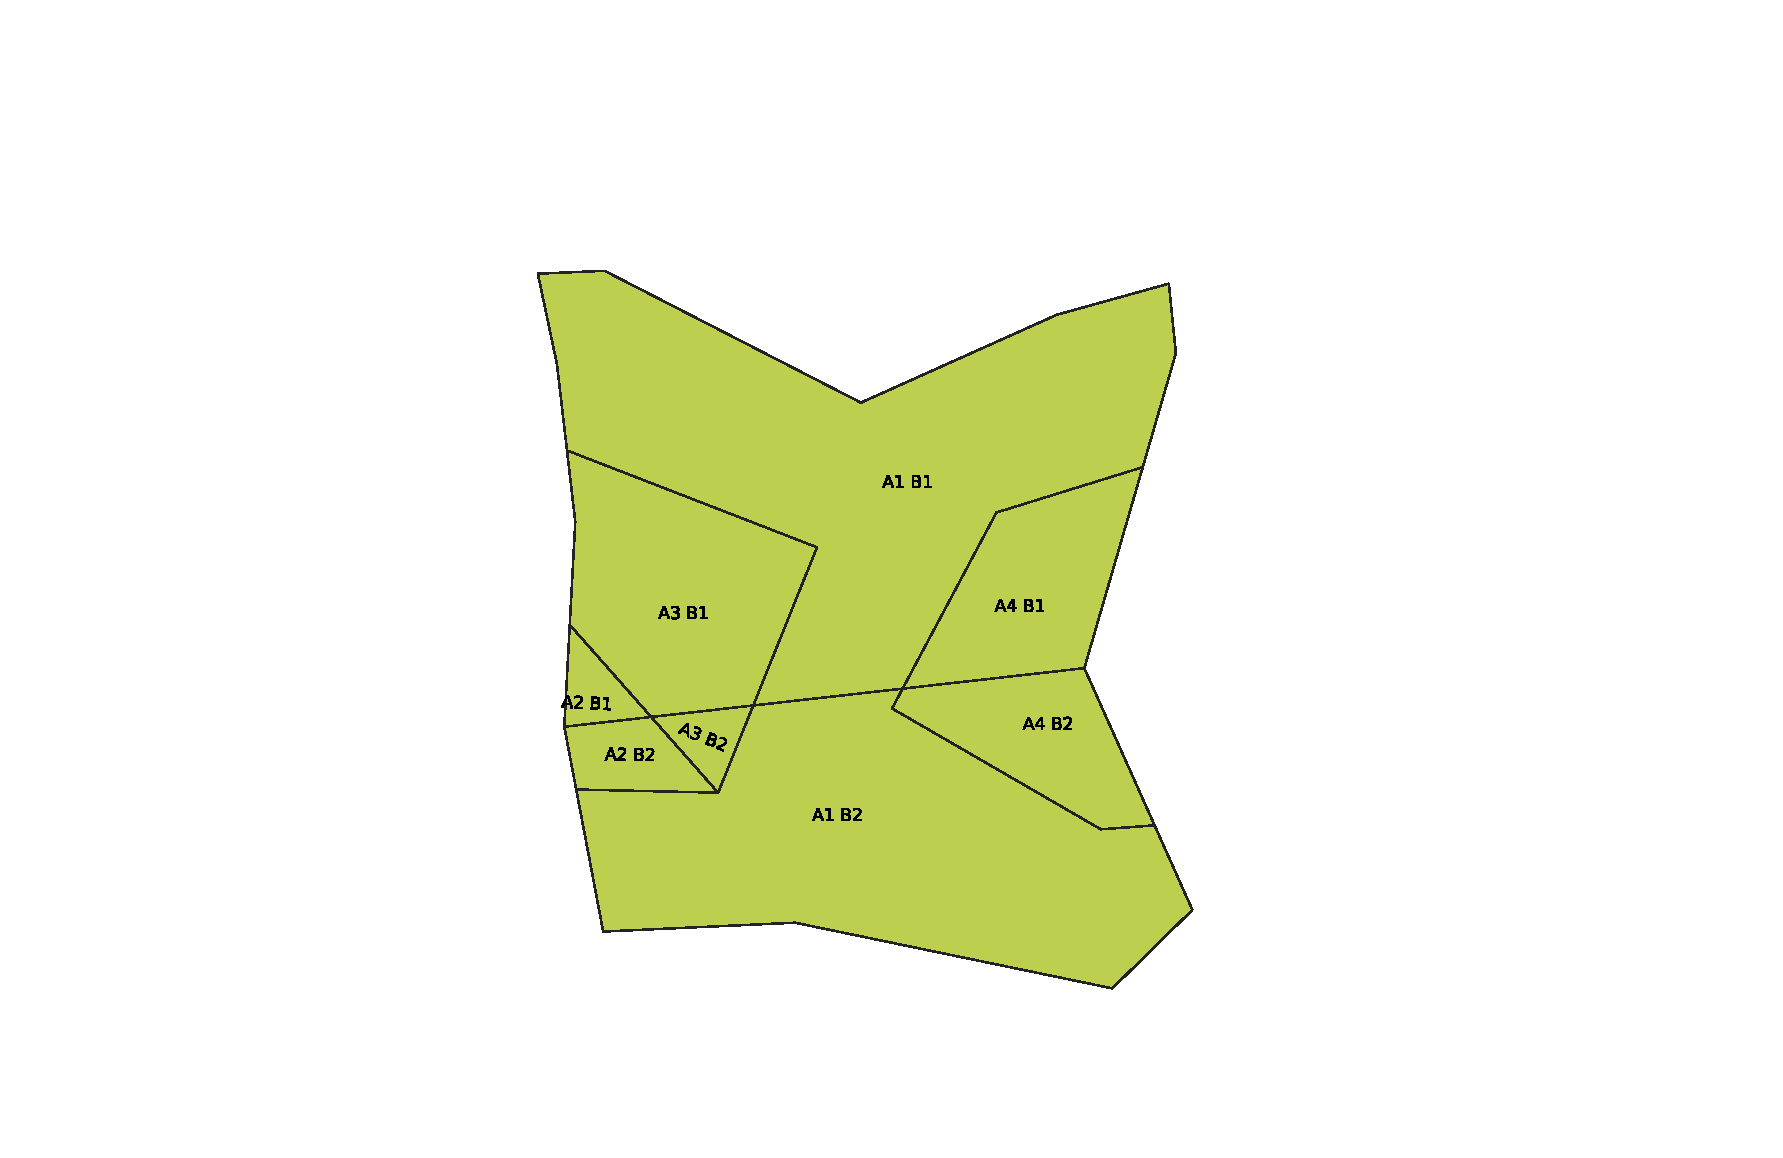
\includegraphics[trim=3cm 0cm 2cm 0cm, clip, width=0.75\linewidth]{figures/Holes04} 
\end{frame}
\begin{frame}{Symmetric difference}
    \centering 
    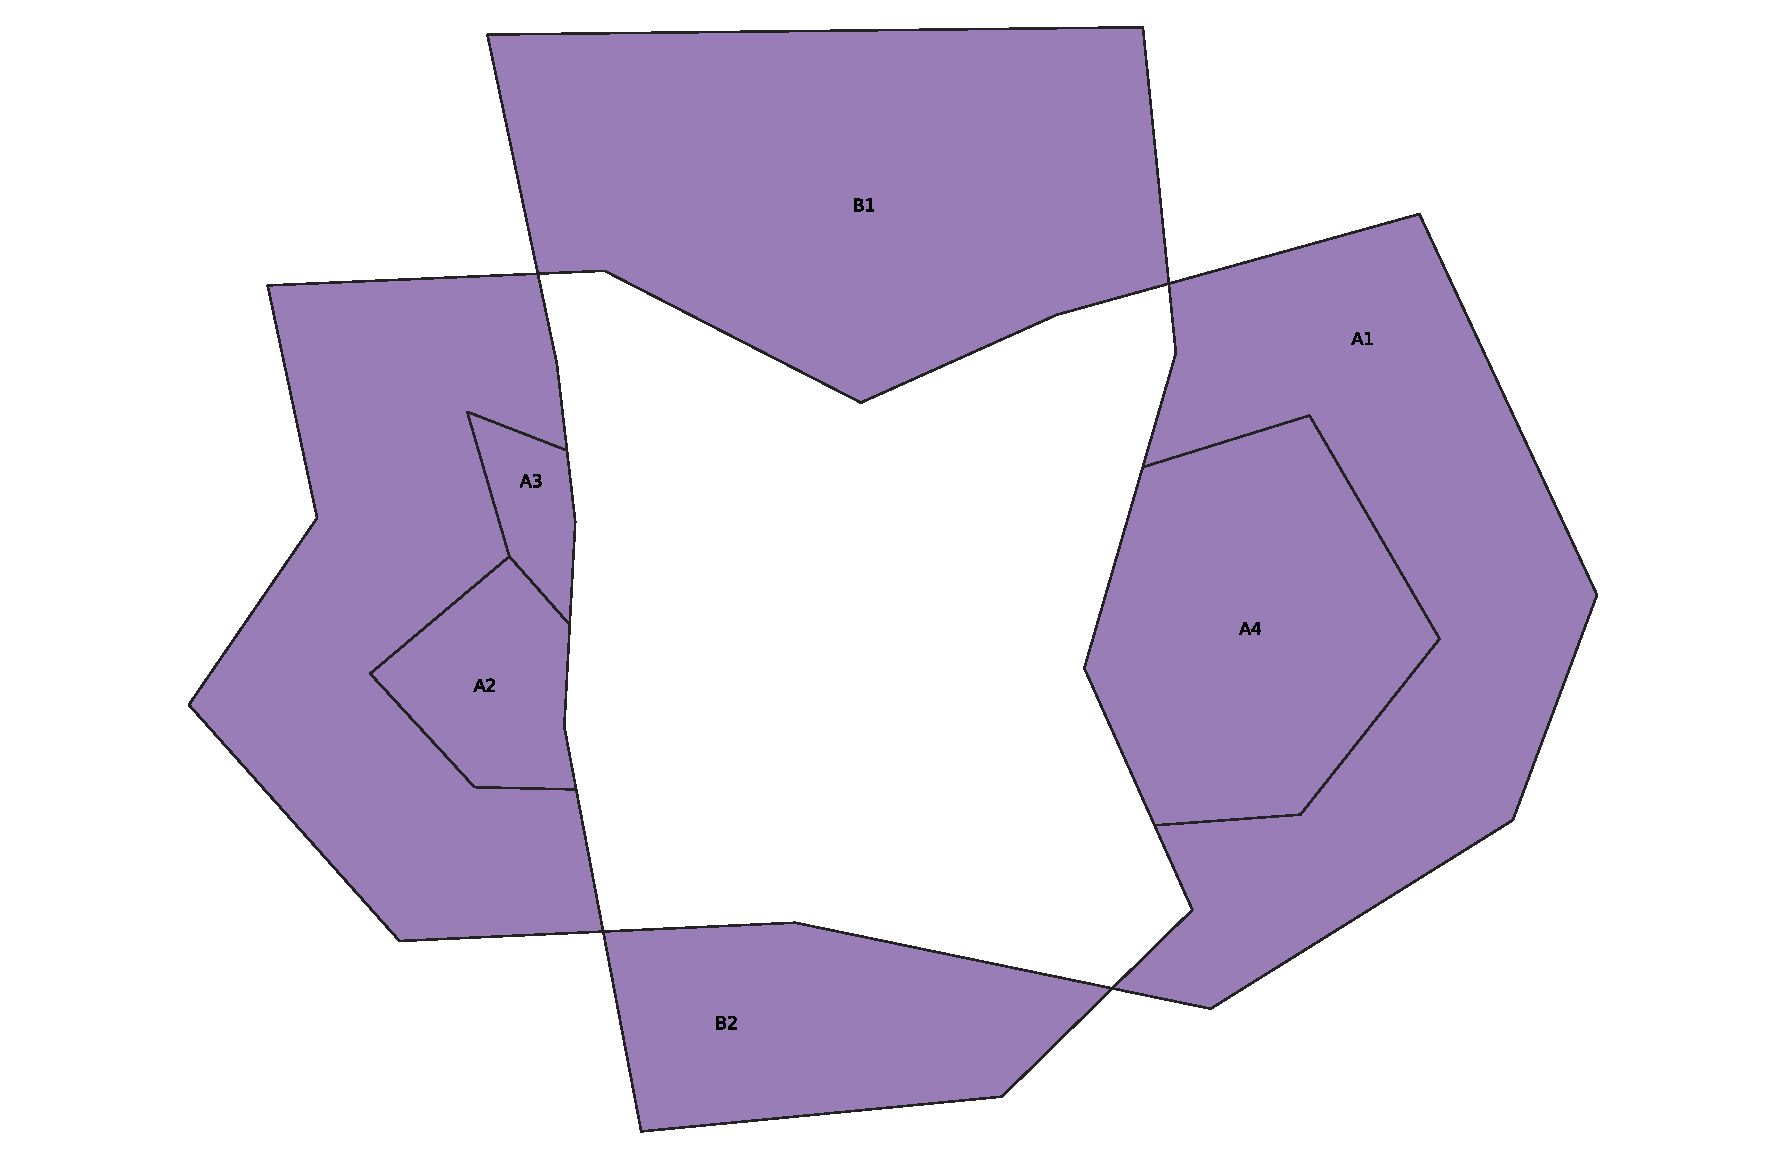
\includegraphics[trim=3cm 0cm 2cm 0cm, clip, width=0.75\linewidth]{figures/Holes05} 
\end{frame}

\begin{frame}{What is next...}
    \begin{itemize}
        \item Perform more tests with holes and multipolygons.
        \item Perform experiments with larger datasets.
    \end{itemize}
\end{frame}

\end{document}
